\documentclass[a4paper]{article}

\usepackage[portuguese]{babel}
\usepackage{comment}
\usepackage[T1]{fontenc}
\usepackage[utf8]{inputenc}
\usepackage{hyperref}
\usepackage{graphicx}
\usepackage{float}
\usepackage{multirow}
\usepackage[hypcap]{caption} % makes \ref point to top of figures and tables
\usepackage{amsmath}
\usepackage[usenames,dvipsnames,svgnames,table]{xcolor}
\usepackage{rotating}

\begin{document}

\begin{titlepage}

	\begin{center}

		\includegraphics[width=6cm]{./title}\\[3cm]

		\textsc{\LARGE Electrónica de Computadores}\\[1.5cm]

		\textsc{\Large Projecto 2}\\[1.5cm]


		{ \huge \bfseries Processamento de Imagem no Processador Softcore MicroBlaze\\[2.5cm] }


		\noindent
		\begin{center} \large
			Gonçalo Ribeiro, 73294\\[5mm]

			Ricardo Amendoeira, 73373\\[5mm]

			Rafael Gonçalves, 73786\\[2.5cm]

			\textit{Docente: Prof. Francisco Alegria}

		\end{center}

		\vfill

		{\large \today}

	\end{center}

\end{titlepage}

\tableofcontents
\pagebreak

\section{Comunicação}

\subsection{PC - PIC: USB}
A comunicação implementada entre o PC e o PIC utilizou a interface USB (Universal Serial Bus).

\subsection{PIC - Sensor: SPI half-duplex}
O método de comunicação utilizado pelo sensor é SPI (Serial Peripheral Interface), que inclui as variantes Full-Duplex e Half-Duplex, ambas permitem a comunicação entre um único Master e vários Slaves.
No caso do sensor a variante utilizada é Half-Duplex que tem como diferenças principais comparado ao Full-Duplex a utilização de menos um porto (para um total de 3) com a desvantagem de não permitir comunicação bidireccional simultânea como o Full-Duplex.
\begin{figure}[H]
\centering

\caption{Imagem pretty de SPI half duplex}
\label{fig:Cherry_box}
\end{figure}

\subsubsection{Explicação do SPI Half-Duplex}  
A variante Half-Duplex usa os seguintes portos:
\begin{enumerate}
    \item SS $\rightarrow$ Slave Select: Quando posto a Low activa o Slave (porto controlado apenas pelo Master)
    \item MSIO $\rightarrow$ Master Slave Input Output: porto de envio/recepção de dados (controlado por ambos mas não em simultâneo)
    \item SCLK $\rightarrow$ Slave Clock: O relógio usado pelo Slave (porto controlado apenas pelo Master)
\end{enumerate}

Para efectuar uma comunicação o Master (no caso do projecto é o PIC) coloca o porto SS a Low para activar o Slave (que neste caso é o sensor), gera um sinal de relógio no porto SCLK e envia a informação bit a bit para o Slave.

Especificamente entre o PIC e o sensor as comunicações são feitas por bytes (ou seja, tanto o PIC como o sensor enviam e esperam receber um byte completo)




\section{Estratégias}
Durante o laboratório, efectuámos alterações iterativas ao código que nos foi fornecido de maneira a implementar as funcionalidades pretendidas.

\subsection{Rato}

\subsubsection{1ª Iteração}
Processos de actualização da posição do cursor:
\begin{enumerate}
    \item PC $\rightarrow$ PIC: um pedido de leitura do registo 3 ($\Delta x$) via USB
    \item PIC $\rightarrow$ Sensor: o endereço do registo (\texttt{0x03}) a ser lido via SPI Half-duplex
    \item Sensor $\rightarrow$ PIC: o valor contido no registo \texttt{0x03} via SPI Half-duplex
    \item PIC $\rightarrow$ PC: o valor lido do sensor, que corresponde a $\Delta x$, via USB
    \item PC $\rightarrow$ PIC: um pedido de leitura do registo 4 ($\Delta y$) via USB
    \item PIC $\rightarrow$ Sensor: o endereço do registo (\texttt{0x04}) a ser lido via SPI Half-duplex
    \item Sensor $\rightarrow$ PIC: o valor contido no registo \texttt{0x04} via SPI Half-duplex
    \item PIC $\rightarrow$ PC: o valor lido do sensor, que corresponde a $\Delta y$, via USB
    \item PC: As variações nas posições são adicionadas às coordenadas actuais do rato.
\end{enumerate}

Formato dos pacotes de dados:

\begin{figure}[H]
\centering
\setlength{\unitlength}{1mm}
\begin{picture}(120,10)
\multiput(0,0)(40,0){4}{\line(0,1){10}}
\multiput(0,0)(0,10){2}{\line(1,0){120}}
\put(0,0){\makebox(40,10){\parbox{4cm}{\centering\texttt{Byte 0: Comando de Leitura}}}}

\put(40,0){\makebox(40,10){\parbox{4cm}{\centering\texttt{Byte 1: Endereço a Ler}}}}

\put(80,0){\makebox(40,10){\parbox{4cm}{\centering\texttt{Byte 2: Comprimento da Resposta}}}}
\end{picture}
\caption{Pacote PC $\rightarrow$ PIC}
\label{pack_pc_pic_1}
\end{figure}

\begin{figure}[H]
\centering
\setlength{\unitlength}{1mm}
\begin{picture}(120,10)
\put(0,0){\line(0,1){10}}
\multiput(90,0)(30,0){2}{\line(0,1){10}}
\multiput(0,0)(0,10){2}{\line(1,0){120}}
\put(0,0){\makebox(90,10){\texttt{Bytes 0-2: Mensagem Original}}}
\put(90,0){\makebox(30,9){\parbox{3cm}{\footnotesize\centering\texttt{Byte 3: Conteúdo do Registo}}}}
\end{picture}
\caption{Pacote PIC $\rightarrow$ PC}
\label{pack_pic_pc_1}
\end{figure}

No entanto, esta abordagem mostrou-se muito lenta, isto é, o rato ``soluçava'' pelo ecrã. Foi determinado que o processo que mais tempo gasta é a comunicação via USB, e, como tal, o código foi adaptado de maneira a diminuir estas comunicações.

\pagebreak

\subsubsection{2ª Iteração}
Processos de actualização da posição do cursor:
\begin{enumerate}
    \item PC $\rightarrow$ PIC: um pedido de leitura dos registo 3 e 4($\Delta x$ e $\Delta y$) via USB
    \item PIC $\rightarrow$ Sensor: o endereço do registo (\texttt{0x03}) a ser lido via SPI Half-duplex
    \item Sensor $\rightarrow$ PIC: o valor contido no registo \texttt{0x03} via SPI Half-duplex
    \item PIC $\rightarrow$ Sensor: o endereço do registo (\texttt{0x04}) a ser lido via SPI Half-duplex
    \item Sensor $\rightarrow$ PIC: o valor contido no registo \texttt{0x04} via SPI Half-duplex
    \item PIC $\rightarrow$ PC: os valores lidos do sensor, que correspondem a $\Delta x$ e $\Delta y$, via USB
    \item PC: As variações nas posições são adicionadas às coordenadas actuais do rato.
\end{enumerate}

Formato dos pacotes de dados:

\begin{figure}[H]
\centering
\setlength{\unitlength}{1mm}
\begin{picture}(120,10)
\multiput(0,0)(60,0){3}{\line(0,1){10}}
\multiput(0,0)(0,10){2}{\line(1,0){120}}
\put(0,0){\makebox(60,10){\parbox{4cm}{\centering\texttt{Byte 0: Comando de Leitura Personalizado}}}}
\put(60,0){\makebox(60,9){\parbox{4cm}{\centering\texttt{Byte 1: Comprimento da Resposta}}}}
\end{picture}
\caption{Pacote PC $\rightarrow$ PIC}
\label{pack_pc_pic_2}
\end{figure}

\begin{figure}[H]
\centering
\setlength{\unitlength}{1mm}
\begin{picture}(120,10)
\put(0,0){\line(0,1){10}}
\multiput(60,0)(30,0){3}{\line(0,1){10}}
\multiput(0,0)(0,10){2}{\line(1,0){120}}
\put(0,0){\makebox(60,10){\parbox{6cm}{\centering\texttt{Bytes 0-1: Mensagem Original}}}}
\put(60,0){\makebox(30,10){\texttt{Byte 2:} $\Delta x$}}
\put(90,0){\makebox(30,10){\texttt{Byte 3:} $\Delta y$}}
\end{picture}
\caption{Pacote PIC $\rightarrow$ PC}
\label{pack_pic_pc_2}
\end{figure}

\subsection{Captura de Imagem}
\subsubsection{1ª Iteração}
Os processos correspondentes à leitura de cada um dos píxeis na implementação inicial são:
\begin{enumerate}
    \item PC $\rightarrow$ PIC: um pedido de leitura do registo \texttt{0x0b} via USB
    \item PIC $\rightarrow$ Sensor: o endereço do registo \texttt{0x0b} via SPI Half-duplex
    \item Sensor $\rightarrow$ PIC: o valor contido no registo via SPI Half-duplex
    \item PIC $\rightarrow$ PC: uma mensagem com o valor lido do registo
    \item PC: Mapeamento dos dados recebidos para um rectângulo no ecrã.
\end{enumerate}

Esta abordagem permite-nos mostrar uma imagem a aproximadamente cada 15 segundos, isto é, muito longe da solução em tempo-real pretendida.

\subsubsection{2ª Iteração}
De maneira a diminuir o número de comunicações USB por cada imagem, a solução mais evidente é incluir mais que um píxel por cada intercâmbio de comunicações.

Uma vez que os pacotes já implementados no código fornecido estão limitados a 64 bytes, foram adaptados de maneira a cada pacote PIC $\rightarrow$ PC conter os dados de 45 píxeis, isto é, 3 colunas da imagem.

\begin{figure}[H]
\centering
\setlength{\unitlength}{0,5mm}
\begin{picture}(150,150)
\multiput(0,0)(10,0){16}{\line(0,1){150}}
\multiput(0,0)(0,10){16}{\line(1,0){150}}
\multiput(2,2)(30,0){5}{\color{red} \line(0,1){146}}
\multiput(2,2)(30,0){5}{\color{red} \line(1,0){26}}
\multiput(28,2)(30,0){5}{\color{red} \line(0,1){146}}
\multiput(2,148)(30,0){5}{\color{red} \line(1,0){26}}
\put(0,0){\makebox(30,150){\color{red} \rotatebox{90}{\LARGE Pacote 5}}}
\put(30,0){\makebox(30,150){\color{red} \rotatebox{90}{\LARGE Pacote 4}}}
\put(60,0){\makebox(30,150){\color{red} \rotatebox{90}{\LARGE Pacote 3}}}
\put(90,0){\makebox(30,150){\color{red} \rotatebox{90}{\LARGE Pacote 2}}}
\put(120,0){\makebox(30,150){\color{red} \rotatebox{90}{\LARGE Pacote 1}}}
\end{picture}
\caption{Divisão da imagem em troços}
\label{picture_layout}
\end{figure}

Ao fazer esta alteração, havia conjuntos verticais de píxeis, de número arbitrário, com exactamente a mesma cor. O mesmo não se verifica na versão anterior do programa.

Ao eliminar as sucessivas comunicações entre PC e PIC, não há tempo para o circuito do sensor capturar um píxel válido. Uma vez que não era feita a verificação da validade do píxel, os valores eram repetidos, criando os padrões de píxeis em colunas.

\subsubsection{3ª Iteração}

Bastou-nos adaptar o código do micro-controlador para fazer uma verificação do bit de validade antes de ler o píxel seguinte para que a imagem aparecesse correctamente.

\begin{figure}[H]
\centering
\setlength{\unitlength}{1mm}
\begin{picture}(120,10)
\multiput(0,0)(120,0){2}{\line(0,1){10}}
\multiput(0,0)(0,10){2}{\line(1,0){120}}
\put(20,0){\line(0,1){10}}
\put(0,0){\makebox(20,9){\parbox{2cm}{\centering\footnotesize\texttt{Bytes 0-1: Mensagem Original}}}}
\put(20,0){\makebox(100,9){\texttt{Bytes 2-46: Bytes de píxeis}}}
\end{picture}
\caption{Pacote PIC $\rightarrow$ PC}
\label{pack_pic_pc_3}
\end{figure}

\subsection{Cursor e Captura de Imagem Simultâneos}

Uma vez constatado que o processo mais demorado é a comunicação via USB, foi decidido não repetir o mesmo erro uma vez mais. Assim, o formato do pacote de dados foi alterado de maneira a incluir os valores de $\Delta x$ e $\Delta y$, para além dos 45 píxeis da imagem a mostrar.

\begin{figure}[H]
\centering
\setlength{\unitlength}{1mm}
\begin{picture}(120,10)
\multiput(0,0)(120,0){2}{\line(0,1){10}}
\multiput(0,0)(0,10){2}{\line(1,0){120}}
\multiput(20,0)(80,0){2}{\line(0,1){10}}
\put(0,0){\makebox(20,9){\parbox{2cm}{\centering\footnotesize\texttt{Bytes 0-1: Mensagem Original}}}}
\put(20,0){\makebox(80,9){\texttt{Bytes 2-46: Bytes de píxeis}}}
\put(100,0){\makebox(20,9){\parbox{2cm}{\centering\footnotesize\texttt{Bytes 47-48: $\Delta x$\texttt{ and }$\Delta y$}}}}
\end{picture}
\caption{Pacote PIC $\rightarrow$ PC}
\label{pack_pic_pc_4}
\end{figure}

\pagebreak
\section{Conclusões}

Os resultados finais foram os esperados. O rato e a imagem são actualizados em simultâneo, sendo que a posição do rato é actulizada 5 vezes por cada actulização total da imagem.

A área que o rato permite capturar é muito reduzida, menor que de 1 $mm^2$. Pudemos constatar isto ao capturar a imagem de um \textregistered\ de dimensão muito reduzida que existe num selo das caixas dos ratos ao lado da marca Cherry GmbH, que se pode ser na Figura~\ref{fig:Cherry_box}. O \textregistered\ tinha o tamanho máximo que o rato conseguia capturar. A imagem capturada pelo rato pode ser vista na Figura~\ref{fig:registed_capture}.

\begin{figure}[b]
\centering

\caption{Selo da caixa do rato, com \textregistered\ assinalado}
\label{fig:Cherry_box}
\end{figure}

\begin{figure}[t]
\centering
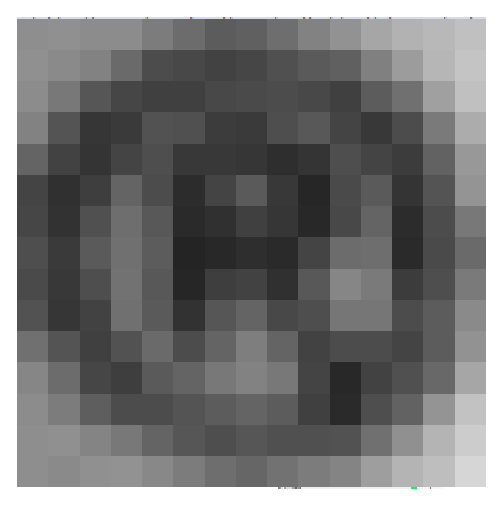
\includegraphics{rprintscreen}
\caption{imagem do \textregistered\ da Figura~\ref{fig:Cherry_box} capturada pelo rato}
\label{fig:registed_capture}
\end{figure}

Alterar a resolução do rato produziu também o efeito esperado: ao reduzirmos a resolução o rato move-se mais rapidamente no ecrã.

Em geral o movimento do rato devia ser um pouco mais rápido para se aproximar da velocidade normal de um rato. A imagem capturada demora um pouco a ser actulizada mas é rápida o suficiente para se conseguir perceber sobre o que é que o rato está a passar quando é movido.

\end{document}